\documentclass[10pt]{article}
\usepackage{ctex}
\usepackage{CJK}
\usepackage{graphicx}
\bibliographystyle{plain}
\setlength{\parindent}{2em}
\begin{document}
\title{Optical systems}
\author{Qilei Zhang}
\date{may 25 2018}
\maketitle
\par
\section{Bistable ring laser}
A ring laser consists of a ring interferometer formed by three or more mirrors and a laser medium inside the cavity. In two-mode ring lasers, the light can travel in a clockwise or counterclockwise direction. Bistability with respect to the direction has been discussed in large detail��see, for example, Man-el, Roy, and Singh . Random switching of the beam intensities, initiated by spontaneous emission in the laser medium and fluctuations in the pump mechanism, indicates bistable operation of the ring laser.\cite{Buensalido2016A}
\par
\begin{figure}[htbp]
\small
\centering
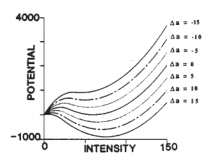
\includegraphics[width=20em]{123.png}
\caption{Bistable ring laser}
\label{fig:lable}
\end{figure}
\section{Lasers with saturable absorbers}
A laser with a saturable absorber is a quantum device consisting of a laser cavity where an amplifying as well as an absorbing medium are placed.\cite{Li2018Flood}
\section{Model for absorptive optical bistability}
Consider a ring interferometer with a passive medium placed in it. Light is coupled into the interferometer through a semipermeable mirror and, likewise, light is transmitted at another mirror. Measuring the intensity of the transmitted wave against the intensity of the incident wave, one finds an S-shaped curve.\cite{Zhang2014An}\\
$X(t)=-H(t)\sum_{n=1}^\infty g_n l_n exp(-l_n t)$\\
$\quad x'=x-x^3+u(t)+A_0 cos(st)$
\bibliography{zaq}
\end{document}

